\documentclass[twoside]{book}

% Packages required by doxygen
\usepackage{fixltx2e}
\usepackage{calc}
\usepackage{doxygen}
\usepackage[export]{adjustbox} % also loads graphicx
\usepackage{graphicx}
\usepackage[utf8]{inputenc}
\usepackage{makeidx}
\usepackage{multicol}
\usepackage{multirow}
\PassOptionsToPackage{warn}{textcomp}
\usepackage{textcomp}
\usepackage[nointegrals]{wasysym}
\usepackage[table]{xcolor}

% Font selection
\usepackage[T1]{fontenc}
\usepackage[scaled=.90]{helvet}
\usepackage{courier}
\usepackage{amssymb}
\usepackage{sectsty}
\renewcommand{\familydefault}{\sfdefault}
\allsectionsfont{%
  \fontseries{bc}\selectfont%
  \color{darkgray}%
}
\renewcommand{\DoxyLabelFont}{%
  \fontseries{bc}\selectfont%
  \color{darkgray}%
}
\newcommand{\+}{\discretionary{\mbox{\scriptsize$\hookleftarrow$}}{}{}}

% Page & text layout
\usepackage{geometry}
\geometry{%
  a4paper,%
  top=2.5cm,%
  bottom=2.5cm,%
  left=2.5cm,%
  right=2.5cm%
}
\tolerance=750
\hfuzz=15pt
\hbadness=750
\setlength{\emergencystretch}{15pt}
\setlength{\parindent}{0cm}
\setlength{\parskip}{3ex plus 2ex minus 2ex}
\makeatletter
\renewcommand{\paragraph}{%
  \@startsection{paragraph}{4}{0ex}{-1.0ex}{1.0ex}{%
    \normalfont\normalsize\bfseries\SS@parafont%
  }%
}
\renewcommand{\subparagraph}{%
  \@startsection{subparagraph}{5}{0ex}{-1.0ex}{1.0ex}{%
    \normalfont\normalsize\bfseries\SS@subparafont%
  }%
}
\makeatother

% Headers & footers
\usepackage{fancyhdr}
\pagestyle{fancyplain}
\fancyhead[LE]{\fancyplain{}{\bfseries\thepage}}
\fancyhead[CE]{\fancyplain{}{}}
\fancyhead[RE]{\fancyplain{}{\bfseries\leftmark}}
\fancyhead[LO]{\fancyplain{}{\bfseries\rightmark}}
\fancyhead[CO]{\fancyplain{}{}}
\fancyhead[RO]{\fancyplain{}{\bfseries\thepage}}
\fancyfoot[LE]{\fancyplain{}{}}
\fancyfoot[CE]{\fancyplain{}{}}
\fancyfoot[RE]{\fancyplain{}{\bfseries\scriptsize Generated by Doxygen }}
\fancyfoot[LO]{\fancyplain{}{\bfseries\scriptsize Generated by Doxygen }}
\fancyfoot[CO]{\fancyplain{}{}}
\fancyfoot[RO]{\fancyplain{}{}}
\renewcommand{\footrulewidth}{0.4pt}
\renewcommand{\chaptermark}[1]{%
  \markboth{#1}{}%
}
\renewcommand{\sectionmark}[1]{%
  \markright{\thesection\ #1}%
}

% Indices & bibliography
\usepackage{natbib}
\usepackage[titles]{tocloft}
\setcounter{tocdepth}{3}
\setcounter{secnumdepth}{5}
\makeindex

% Hyperlinks (required, but should be loaded last)
\usepackage{ifpdf}
\ifpdf
  \usepackage[pdftex,pagebackref=true]{hyperref}
\else
  \usepackage[ps2pdf,pagebackref=true]{hyperref}
\fi
\hypersetup{%
  colorlinks=true,%
  linkcolor=blue,%
  citecolor=blue,%
  unicode%
}

% Custom commands
\newcommand{\clearemptydoublepage}{%
  \newpage{\pagestyle{empty}\cleardoublepage}%
}

\usepackage{caption}
\captionsetup{labelsep=space,justification=centering,font={bf},singlelinecheck=off,skip=4pt,position=top}

%===== C O N T E N T S =====

\begin{document}

% Titlepage & ToC
\hypersetup{pageanchor=false,
             bookmarksnumbered=true,
             pdfencoding=unicode
            }
\pagenumbering{roman}
\begin{titlepage}
\vspace*{7cm}
\begin{center}%
{\Large Target parser }\\
\vspace*{1cm}
{\large Generated by Doxygen 1.8.11}\\
\end{center}
\end{titlepage}
\clearemptydoublepage
\tableofcontents
\clearemptydoublepage
\pagenumbering{arabic}
\hypersetup{pageanchor=true}

%--- Begin generated contents ---
\chapter{Module Index}
\section{Modules}
Here is a list of all modules\+:\begin{DoxyCompactList}
\item \contentsline{section}{Target\+Parser}{\pageref{group__TargetParser}}{}
\end{DoxyCompactList}

\chapter{Namespace Index}
\section{Namespace List}
Here is a list of all documented namespaces with brief descriptions\+:\begin{DoxyCompactList}
\item\contentsline{section}{\hyperlink{namespacetarget__parser}{target\+\_\+parser} \\*Содержит функции и структуры для работы с парсером }{\pageref{namespacetarget__parser}}{}
\end{DoxyCompactList}

\chapter{Class Index}
\section{Class List}
Here are the classes, structs, unions and interfaces with brief descriptions\+:\begin{DoxyCompactList}
\item\contentsline{section}{\hyperlink{classtarget__parser_1_1PatternTree}{target\+\_\+parser\+::\+Pattern\+Tree} \\*Класс представляющий разобранное выражение в виде дерева, возвращается из метода \hyperlink{namespacetarget__parser_a3e0ffa10d4fd38f05986d81c0529fdc1}{Parse } }{\pageref{classtarget__parser_1_1PatternTree}}{}
\item\contentsline{section}{\hyperlink{structtarget__parser_1_1Vertex}{target\+\_\+parser\+::\+Vertex} \\*класс представляющий терминальное состояние вершины в дереве разбора \hyperlink{classtarget__parser_1_1PatternTree}{Pattern\+Tree} }{\pageref{structtarget__parser_1_1Vertex}}{}
\end{DoxyCompactList}

\chapter{File Index}
\section{File List}
Here is a list of all documented files with brief descriptions\+:\begin{DoxyCompactList}
\item\contentsline{section}{/home/nemchenko/work/tasks/sorm/sorm-\/probe/lib/\+Target\+Parser/include/\hyperlink{InitTargetParser_8h}{Init\+Target\+Parser.\+h} \\*содержит структуру Vertex и декларацию функции \hyperlink{namespacetarget__parser_aabf89c1d99b04bac59515c8616155d94}{target\+\_\+parser\+::\+Init} }{\pageref{InitTargetParser_8h}}{}
\item\contentsline{section}{/home/nemchenko/work/tasks/sorm/sorm-\/probe/lib/\+Target\+Parser/include/\hyperlink{Parser_8h}{Parser.\+h} \\*содержит декларации функций для парсинга \hyperlink{namespacetarget__parser_a3e0ffa10d4fd38f05986d81c0529fdc1}{target\+\_\+parser\+::\+Parse(char const $\ast$, size\+\_\+t, int $\ast$)} }{\pageref{Parser_8h}}{}
\item\contentsline{section}{/home/nemchenko/work/tasks/sorm/sorm-\/probe/lib/\+Target\+Parser/include/\hyperlink{PatternTree_8h}{Pattern\+Tree.\+h} \\*содержит класс представляющий дерево разбора \hyperlink{classtarget__parser_1_1PatternTree}{target\+\_\+parser\+::\+Pattern\+Tree} }{\pageref{PatternTree_8h}}{}
\end{DoxyCompactList}

\chapter{Module Documentation}
\hypertarget{group__TargetParser}{}\section{Target\+Parser}
\label{group__TargetParser}\index{Target\+Parser@{Target\+Parser}}


содержит функции для парсинга и структуры для работы с разобранным деревом  


\subsection*{Files}
\begin{DoxyCompactItemize}
\item 
file \hyperlink{InitTargetParser_8h}{Init\+Target\+Parser.\+h}
\begin{DoxyCompactList}\small\item\em содержит структуру Vertex и декларацию функции \hyperlink{namespacetarget__parser_aabf89c1d99b04bac59515c8616155d94}{target\+\_\+parser\+::\+Init}. \end{DoxyCompactList}\item 
file \hyperlink{Parser_8h}{Parser.\+h}
\begin{DoxyCompactList}\small\item\em содержит декларации функций для парсинга \hyperlink{namespacetarget__parser_a3e0ffa10d4fd38f05986d81c0529fdc1}{target\+\_\+parser\+::\+Parse(char const $\ast$, size\+\_\+t, int $\ast$)} \end{DoxyCompactList}\item 
file \hyperlink{PatternTree_8h}{Pattern\+Tree.\+h}
\begin{DoxyCompactList}\small\item\em содержит класс представляющий дерево разбора \hyperlink{classtarget__parser_1_1PatternTree}{target\+\_\+parser\+::\+Pattern\+Tree}. \end{DoxyCompactList}\end{DoxyCompactItemize}
\subsection*{Namespaces}
\begin{DoxyCompactItemize}
\item 
 \hyperlink{namespacetarget__parser}{target\+\_\+parser}
\begin{DoxyCompactList}\small\item\em Содержит функции и структуры для работы с парсером \end{DoxyCompactList}\end{DoxyCompactItemize}


\subsection{Detailed Description}
содержит функции для парсинга и структуры для работы с разобранным деревом 

\begin{DoxyVerb}Пример валидной строки для разбора:
  ip = "123*" | host = "?google.\"ru" & !(imsdn = "10" & email = "*gmail" | phone = "*952*")

Грамматика парсера:
  Expression     = OrPart ('|' OrPart)*
  OrPart         = AndPart ('&' AndPart)*
  AndPart        =  '!' Symbols | Symbols
  Symbols        = '('  Expression  ')' | Terminal
  Terminal       = pattern_name '=' quoted_pattern
  quoted_pattern = '"' ( ('\' anychar) | (anychar - '"') )* '"'
  pattern_name   = [a-z_]+
  ws             = (' ')*
\end{DoxyVerb}


в main нужно подключить файл \hyperlink{InitTargetParser_8h}{Init\+Target\+Parser.\+h} и вызвать функцию \hyperlink{namespacetarget__parser_aabf89c1d99b04bac59515c8616155d94}{target\+\_\+parser\+::\+Init()} ~\newline
 в месте, где нужно распарсить, подключать файл \hyperlink{Parser_8h}{Parser.\+h} и вызывать функцию и \hyperlink{namespacetarget__parser_a3e0ffa10d4fd38f05986d81c0529fdc1}{target\+\_\+parser\+::\+Parse(char const $\ast$, size\+\_\+t, int $\ast$)}

\begin{DoxyAuthor}{Author}
Nemchenko Eugene 
\end{DoxyAuthor}
\begin{DoxyDate}{Date}
12/08/2016 
\end{DoxyDate}

\chapter{Namespace Documentation}
\hypertarget{namespacetarget__parser}{}\section{target\+\_\+parser Namespace Reference}
\label{namespacetarget__parser}\index{target\+\_\+parser@{target\+\_\+parser}}


Содержит функции и структуры для работы с парсером  


\subsection*{Classes}
\begin{DoxyCompactItemize}
\item 
class \hyperlink{classtarget__parser_1_1PatternTree}{Pattern\+Tree}
\begin{DoxyCompactList}\small\item\em Класс представляющий разобранное выражение в виде дерева, возвращается из метода \hyperlink{namespacetarget__parser_a3e0ffa10d4fd38f05986d81c0529fdc1}{Parse }. \end{DoxyCompactList}\item 
struct \hyperlink{structtarget__parser_1_1Vertex}{Vertex}
\begin{DoxyCompactList}\small\item\em класс представляющий терминальное состояние вершины в дереве разбора \hyperlink{classtarget__parser_1_1PatternTree}{Pattern\+Tree}. \end{DoxyCompactList}\end{DoxyCompactItemize}
\subsection*{Typedefs}
\begin{DoxyCompactItemize}
\item 
typedef std\+::function$<$ void(const \hyperlink{structtarget__parser_1_1Vertex}{Vertex} \&)$>$ \hyperlink{namespacetarget__parser_aa28dbbced739f360834455cbffeaa6e4}{Func}\hypertarget{namespacetarget__parser_aa28dbbced739f360834455cbffeaa6e4}{}\label{namespacetarget__parser_aa28dbbced739f360834455cbffeaa6e4}

\begin{DoxyCompactList}\small\item\em тип функтора который передается в метод \hyperlink{classtarget__parser_1_1PatternTree_a851ee4b1279c2dcfc4557cab03f8aa83}{Pattern\+Tree\+::\+For\+Each\+Vertex}. \end{DoxyCompactList}\end{DoxyCompactItemize}
\subsection*{Functions}
\begin{DoxyCompactItemize}
\item 
void \hyperlink{namespacetarget__parser_aabf89c1d99b04bac59515c8616155d94}{Init} ()\hypertarget{namespacetarget__parser_aabf89c1d99b04bac59515c8616155d94}{}\label{namespacetarget__parser_aabf89c1d99b04bac59515c8616155d94}

\begin{DoxyCompactList}\small\item\em инициализирует грамматику и парсер, нужно вызывать в main до использования функции \hyperlink{namespacetarget__parser_a3e0ffa10d4fd38f05986d81c0529fdc1}{Parse }. \end{DoxyCompactList}\item 
\hyperlink{classtarget__parser_1_1PatternTree}{Pattern\+Tree} \hyperlink{namespacetarget__parser_acbab48610c44fba004e282d8008df094}{Parse} (const std\+::string \&text, int $\ast$pos\+\_\+unparsed=nullptr)
\item 
\hyperlink{classtarget__parser_1_1PatternTree}{Pattern\+Tree} \hyperlink{namespacetarget__parser_a3e0ffa10d4fd38f05986d81c0529fdc1}{Parse} (char const $\ast$first, size\+\_\+t len, int $\ast$pos\+\_\+unparsed=nullptr)
\begin{DoxyCompactList}\small\item\em разбирает строку по соответствующей грамматике и строит для нее дерево разбора \end{DoxyCompactList}\end{DoxyCompactItemize}


\subsection{Detailed Description}
Содержит функции и структуры для работы с парсером 

\subsection{Function Documentation}
\index{target\+\_\+parser@{target\+\_\+parser}!Parse@{Parse}}
\index{Parse@{Parse}!target\+\_\+parser@{target\+\_\+parser}}
\subsubsection[{\texorpdfstring{Parse(const std\+::string \&text, int $\ast$pos\+\_\+unparsed=nullptr)}{Parse(const std::string &text, int *pos_unparsed=nullptr)}}]{\setlength{\rightskip}{0pt plus 5cm}{\bf Pattern\+Tree} target\+\_\+parser\+::\+Parse (
\begin{DoxyParamCaption}
\item[{const std\+::string \&}]{text, }
\item[{int $\ast$}]{pos\+\_\+unparsed = {\ttfamily nullptr}}
\end{DoxyParamCaption}
)}\hypertarget{namespacetarget__parser_acbab48610c44fba004e282d8008df094}{}\label{namespacetarget__parser_acbab48610c44fba004e282d8008df094}
\begin{DoxySeeAlso}{See also}
\hyperlink{namespacetarget__parser_a3e0ffa10d4fd38f05986d81c0529fdc1}{Parse(char const $\ast$, size\+\_\+t, int $\ast$)} 
\end{DoxySeeAlso}
\index{target\+\_\+parser@{target\+\_\+parser}!Parse@{Parse}}
\index{Parse@{Parse}!target\+\_\+parser@{target\+\_\+parser}}
\subsubsection[{\texorpdfstring{Parse(char const $\ast$first, size\+\_\+t len, int $\ast$pos\+\_\+unparsed=nullptr)}{Parse(char const *first, size_t len, int *pos_unparsed=nullptr)}}]{\setlength{\rightskip}{0pt plus 5cm}{\bf Pattern\+Tree} target\+\_\+parser\+::\+Parse (
\begin{DoxyParamCaption}
\item[{char const $\ast$}]{first, }
\item[{size\+\_\+t}]{len, }
\item[{int $\ast$}]{pos\+\_\+unparsed = {\ttfamily nullptr}}
\end{DoxyParamCaption}
)}\hypertarget{namespacetarget__parser_a3e0ffa10d4fd38f05986d81c0529fdc1}{}\label{namespacetarget__parser_a3e0ffa10d4fd38f05986d81c0529fdc1}


разбирает строку по соответствующей грамматике и строит для нее дерево разбора 


\begin{DoxyParams}{Parameters}
{\em first} & указатель на начало строки \\
\hline
{\em len} & длина строки \\
\hline
{\em pos\+\_\+unparsed} & если не равен nullptr, в случае ошибки (\hyperlink{classtarget__parser_1_1PatternTree_a4732f8e97b9e85e7072b21b4e0cb6bbd}{Is\+Valid } == false), указывает на первый неразобранный символ \\
\hline
\end{DoxyParams}
\begin{DoxyReturn}{Returns}
разобранное дерево, нужно проверить его, что он в валидном состоянии(строка распарсилась) 
\end{DoxyReturn}

\chapter{Class Documentation}
\hypertarget{classtarget__parser_1_1PatternTree}{}\section{target\+\_\+parser\+:\+:Pattern\+Tree Class Reference}
\label{classtarget__parser_1_1PatternTree}\index{target\+\_\+parser\+::\+Pattern\+Tree@{target\+\_\+parser\+::\+Pattern\+Tree}}


Класс представляющий разобранное выражение в виде дерева, возвращается из метода \hyperlink{namespacetarget__parser_a3e0ffa10d4fd38f05986d81c0529fdc1}{Parse }.  




{\ttfamily \#include $<$Pattern\+Tree.\+h$>$}

\subsection*{Public Member Functions}
\begin{DoxyCompactItemize}
\item 
{\bfseries Pattern\+Tree} (const \hyperlink{classtarget__parser_1_1PatternTree}{Pattern\+Tree} \&rhs)\hypertarget{classtarget__parser_1_1PatternTree_a2de6f22b3c103c7d6e8ab42d3208ad44}{}\label{classtarget__parser_1_1PatternTree_a2de6f22b3c103c7d6e8ab42d3208ad44}

\item 
\hyperlink{classtarget__parser_1_1PatternTree}{Pattern\+Tree} \& \hyperlink{classtarget__parser_1_1PatternTree_a52d2823b79a76e29e9ddd8d6cadba634}{operator=} (const \hyperlink{classtarget__parser_1_1PatternTree}{Pattern\+Tree} \&rhs)\hypertarget{classtarget__parser_1_1PatternTree_a52d2823b79a76e29e9ddd8d6cadba634}{}\label{classtarget__parser_1_1PatternTree_a52d2823b79a76e29e9ddd8d6cadba634}

\begin{DoxyCompactList}\small\item\em полностью копирует дерево \end{DoxyCompactList}\item 
void \hyperlink{classtarget__parser_1_1PatternTree_a851ee4b1279c2dcfc4557cab03f8aa83}{For\+Each\+Vertex} (const \hyperlink{namespacetarget__parser_aa28dbbced739f360834455cbffeaa6e4}{Func} \&func) const 
\begin{DoxyCompactList}\small\item\em вызывает функцию func на каждой из терминальных вершин дерева, передавая ей состояние вершины \end{DoxyCompactList}\item 
void \hyperlink{classtarget__parser_1_1PatternTree_a931c01fcdabeedc5b6bdf651c544b1ab}{Set\+Value} (int pos, bool value)
\begin{DoxyCompactList}\small\item\em обновляет значение в вершине с номером pos. \end{DoxyCompactList}\item 
bool \hyperlink{classtarget__parser_1_1PatternTree_afb6cc7464f4df5eca028edfb6fd6d222}{Calculate} () const 
\begin{DoxyCompactList}\small\item\em считает значение для всего логического выражения, представленного в виде дерева \end{DoxyCompactList}\item 
std\+::string \hyperlink{classtarget__parser_1_1PatternTree_ab73d10f856192a4e6147c06c383302d1}{To\+String} () const 
\begin{DoxyCompactList}\small\item\em конвертирует дерево в строковое представление, расставляя скобки около всех операций \end{DoxyCompactList}\item 
bool \hyperlink{classtarget__parser_1_1PatternTree_a4732f8e97b9e85e7072b21b4e0cb6bbd}{Is\+Valid} () const 
\begin{DoxyCompactList}\small\item\em возвращает true, в случае если дерево валидно распарсилось и готово к использованию \end{DoxyCompactList}\end{DoxyCompactItemize}
\subsection*{Friends}
\begin{DoxyCompactItemize}
\item 
std\+::ostream \& {\bfseries operator$<$$<$} (std\+::ostream \&out, const \hyperlink{classtarget__parser_1_1PatternTree}{Pattern\+Tree} \&pt)\hypertarget{classtarget__parser_1_1PatternTree_aaaaf63cb27d3e6f0295946db934787cb}{}\label{classtarget__parser_1_1PatternTree_aaaaf63cb27d3e6f0295946db934787cb}

\item 
\hyperlink{classtarget__parser_1_1PatternTree}{Pattern\+Tree} \hyperlink{classtarget__parser_1_1PatternTree_afbef828a1da57a807431665a6be3cfb1}{Parse} (char const $\ast$first, size\+\_\+t len, int $\ast$pos\+\_\+unparsed)
\begin{DoxyCompactList}\small\item\em разбирает строку по соответствующей грамматике и строит для нее дерево разбора \end{DoxyCompactList}\end{DoxyCompactItemize}


\subsection{Detailed Description}
Класс представляющий разобранное выражение в виде дерева, возвращается из метода \hyperlink{namespacetarget__parser_a3e0ffa10d4fd38f05986d81c0529fdc1}{Parse }. 

\subsection{Member Function Documentation}
\index{target\+\_\+parser\+::\+Pattern\+Tree@{target\+\_\+parser\+::\+Pattern\+Tree}!Calculate@{Calculate}}
\index{Calculate@{Calculate}!target\+\_\+parser\+::\+Pattern\+Tree@{target\+\_\+parser\+::\+Pattern\+Tree}}
\subsubsection[{\texorpdfstring{Calculate() const }{Calculate() const }}]{\setlength{\rightskip}{0pt plus 5cm}bool target\+\_\+parser\+::\+Pattern\+Tree\+::\+Calculate (
\begin{DoxyParamCaption}
{}
\end{DoxyParamCaption}
) const}\hypertarget{classtarget__parser_1_1PatternTree_afb6cc7464f4df5eca028edfb6fd6d222}{}\label{classtarget__parser_1_1PatternTree_afb6cc7464f4df5eca028edfb6fd6d222}


считает значение для всего логического выражения, представленного в виде дерева 

\begin{DoxyReturn}{Returns}
значение логического выражения 
\end{DoxyReturn}
\index{target\+\_\+parser\+::\+Pattern\+Tree@{target\+\_\+parser\+::\+Pattern\+Tree}!For\+Each\+Vertex@{For\+Each\+Vertex}}
\index{For\+Each\+Vertex@{For\+Each\+Vertex}!target\+\_\+parser\+::\+Pattern\+Tree@{target\+\_\+parser\+::\+Pattern\+Tree}}
\subsubsection[{\texorpdfstring{For\+Each\+Vertex(const Func \&func) const }{ForEachVertex(const Func &func) const }}]{\setlength{\rightskip}{0pt plus 5cm}void target\+\_\+parser\+::\+Pattern\+Tree\+::\+For\+Each\+Vertex (
\begin{DoxyParamCaption}
\item[{const {\bf Func} \&}]{func}
\end{DoxyParamCaption}
) const}\hypertarget{classtarget__parser_1_1PatternTree_a851ee4b1279c2dcfc4557cab03f8aa83}{}\label{classtarget__parser_1_1PatternTree_a851ee4b1279c2dcfc4557cab03f8aa83}


вызывает функцию func на каждой из терминальных вершин дерева, передавая ей состояние вершины 


\begin{DoxyParams}{Parameters}
{\em func} & функтор который будет вызываться \\
\hline
\end{DoxyParams}
\index{target\+\_\+parser\+::\+Pattern\+Tree@{target\+\_\+parser\+::\+Pattern\+Tree}!Is\+Valid@{Is\+Valid}}
\index{Is\+Valid@{Is\+Valid}!target\+\_\+parser\+::\+Pattern\+Tree@{target\+\_\+parser\+::\+Pattern\+Tree}}
\subsubsection[{\texorpdfstring{Is\+Valid() const }{IsValid() const }}]{\setlength{\rightskip}{0pt plus 5cm}bool target\+\_\+parser\+::\+Pattern\+Tree\+::\+Is\+Valid (
\begin{DoxyParamCaption}
{}
\end{DoxyParamCaption}
) const}\hypertarget{classtarget__parser_1_1PatternTree_a4732f8e97b9e85e7072b21b4e0cb6bbd}{}\label{classtarget__parser_1_1PatternTree_a4732f8e97b9e85e7072b21b4e0cb6bbd}


возвращает true, в случае если дерево валидно распарсилось и готово к использованию 

\begin{DoxyReturn}{Returns}
готовность дерева к использованию 
\end{DoxyReturn}
\index{target\+\_\+parser\+::\+Pattern\+Tree@{target\+\_\+parser\+::\+Pattern\+Tree}!Set\+Value@{Set\+Value}}
\index{Set\+Value@{Set\+Value}!target\+\_\+parser\+::\+Pattern\+Tree@{target\+\_\+parser\+::\+Pattern\+Tree}}
\subsubsection[{\texorpdfstring{Set\+Value(int pos, bool value)}{SetValue(int pos, bool value)}}]{\setlength{\rightskip}{0pt plus 5cm}void target\+\_\+parser\+::\+Pattern\+Tree\+::\+Set\+Value (
\begin{DoxyParamCaption}
\item[{int}]{pos, }
\item[{bool}]{value}
\end{DoxyParamCaption}
)}\hypertarget{classtarget__parser_1_1PatternTree_a931c01fcdabeedc5b6bdf651c544b1ab}{}\label{classtarget__parser_1_1PatternTree_a931c01fcdabeedc5b6bdf651c544b1ab}


обновляет значение в вершине с номером pos. 


\begin{DoxyParams}{Parameters}
{\em pos} & номер вершины, который можно получить при вызове функции \hyperlink{classtarget__parser_1_1PatternTree_a851ee4b1279c2dcfc4557cab03f8aa83}{For\+Each\+Vertex(const Func\& func) const} \\
\hline
{\em value} & новое значение для вершины \\
\hline
\end{DoxyParams}
\index{target\+\_\+parser\+::\+Pattern\+Tree@{target\+\_\+parser\+::\+Pattern\+Tree}!To\+String@{To\+String}}
\index{To\+String@{To\+String}!target\+\_\+parser\+::\+Pattern\+Tree@{target\+\_\+parser\+::\+Pattern\+Tree}}
\subsubsection[{\texorpdfstring{To\+String() const }{ToString() const }}]{\setlength{\rightskip}{0pt plus 5cm}std\+::string target\+\_\+parser\+::\+Pattern\+Tree\+::\+To\+String (
\begin{DoxyParamCaption}
{}
\end{DoxyParamCaption}
) const}\hypertarget{classtarget__parser_1_1PatternTree_ab73d10f856192a4e6147c06c383302d1}{}\label{classtarget__parser_1_1PatternTree_ab73d10f856192a4e6147c06c383302d1}


конвертирует дерево в строковое представление, расставляя скобки около всех операций 

\begin{DoxyReturn}{Returns}
строковое представление дерева 
\end{DoxyReturn}


\subsection{Friends And Related Function Documentation}
\index{target\+\_\+parser\+::\+Pattern\+Tree@{target\+\_\+parser\+::\+Pattern\+Tree}!Parse@{Parse}}
\index{Parse@{Parse}!target\+\_\+parser\+::\+Pattern\+Tree@{target\+\_\+parser\+::\+Pattern\+Tree}}
\subsubsection[{\texorpdfstring{Parse}{Parse}}]{\setlength{\rightskip}{0pt plus 5cm}{\bf Pattern\+Tree} Parse (
\begin{DoxyParamCaption}
\item[{char const $\ast$}]{first, }
\item[{size\+\_\+t}]{len, }
\item[{int $\ast$}]{pos\+\_\+unparsed}
\end{DoxyParamCaption}
)\hspace{0.3cm}{\ttfamily [friend]}}\hypertarget{classtarget__parser_1_1PatternTree_afbef828a1da57a807431665a6be3cfb1}{}\label{classtarget__parser_1_1PatternTree_afbef828a1da57a807431665a6be3cfb1}


разбирает строку по соответствующей грамматике и строит для нее дерево разбора 


\begin{DoxyParams}{Parameters}
{\em first} & указатель на начало строки \\
\hline
{\em len} & длина строки \\
\hline
{\em pos\+\_\+unparsed} & если не равен nullptr, в случае ошибки (\hyperlink{classtarget__parser_1_1PatternTree_a4732f8e97b9e85e7072b21b4e0cb6bbd}{Is\+Valid } == false), указывает на первый неразобранный символ \\
\hline
\end{DoxyParams}
\begin{DoxyReturn}{Returns}
разобранное дерево, нужно проверить его, что он в валидном состоянии(строка распарсилась) 
\end{DoxyReturn}


The documentation for this class was generated from the following file\+:\begin{DoxyCompactItemize}
\item 
/home/nemchenko/work/tasks/sorm/sorm-\/probe/lib/\+Target\+Parser/include/\hyperlink{PatternTree_8h}{Pattern\+Tree.\+h}\end{DoxyCompactItemize}

\hypertarget{structtarget__parser_1_1Vertex}{}\section{target\+\_\+parser\+:\+:Vertex Struct Reference}
\label{structtarget__parser_1_1Vertex}\index{target\+\_\+parser\+::\+Vertex@{target\+\_\+parser\+::\+Vertex}}


класс представляющий терминальное состояние вершины в дереве разбора \hyperlink{classtarget__parser_1_1PatternTree}{Pattern\+Tree}.  




{\ttfamily \#include $<$Init\+Target\+Parser.\+h$>$}

\subsection*{Public Attributes}
\begin{DoxyCompactItemize}
\item 
int \hyperlink{structtarget__parser_1_1Vertex_a314e9edd83acba4cd05bbc9c528d2d16}{vertex\+Id}\hypertarget{structtarget__parser_1_1Vertex_a314e9edd83acba4cd05bbc9c528d2d16}{}\label{structtarget__parser_1_1Vertex_a314e9edd83acba4cd05bbc9c528d2d16}

\begin{DoxyCompactList}\small\item\em уникальный идентификатор вершины \end{DoxyCompactList}\item 
const std\+::string \& \hyperlink{structtarget__parser_1_1Vertex_ae42000f37242f120acfa97bfd4331577}{pattern\+\_\+name}\hypertarget{structtarget__parser_1_1Vertex_ae42000f37242f120acfa97bfd4331577}{}\label{structtarget__parser_1_1Vertex_ae42000f37242f120acfa97bfd4331577}

\begin{DoxyCompactList}\small\item\em имя паттерна ip, email ... \end{DoxyCompactList}\item 
const std\+::string \& \hyperlink{structtarget__parser_1_1Vertex_ae56e40ccbab727eae454847485e78296}{pattern}\hypertarget{structtarget__parser_1_1Vertex_ae56e40ccbab727eae454847485e78296}{}\label{structtarget__parser_1_1Vertex_ae56e40ccbab727eae454847485e78296}

\begin{DoxyCompactList}\small\item\em сам паттерн \end{DoxyCompactList}\end{DoxyCompactItemize}
\subsection*{Friends}
\begin{DoxyCompactItemize}
\item 
std\+::ostream \& \hyperlink{structtarget__parser_1_1Vertex_a4e49de56cff8bdd50a1901814dd4f5c0}{operator$<$$<$} (std\+::ostream \&out, const \hyperlink{structtarget__parser_1_1Vertex}{Vertex} \&v)\hypertarget{structtarget__parser_1_1Vertex_a4e49de56cff8bdd50a1901814dd4f5c0}{}\label{structtarget__parser_1_1Vertex_a4e49de56cff8bdd50a1901814dd4f5c0}

\begin{DoxyCompactList}\small\item\em выводит вершину, для дебага \end{DoxyCompactList}\end{DoxyCompactItemize}


\subsection{Detailed Description}
класс представляющий терминальное состояние вершины в дереве разбора \hyperlink{classtarget__parser_1_1PatternTree}{Pattern\+Tree}. 

The documentation for this struct was generated from the following file\+:\begin{DoxyCompactItemize}
\item 
/home/nemchenko/work/tasks/sorm/sorm-\/probe/lib/\+Target\+Parser/include/\hyperlink{InitTargetParser_8h}{Init\+Target\+Parser.\+h}\end{DoxyCompactItemize}

\chapter{File Documentation}
\hypertarget{InitTargetParser_8h}{}\section{/home/nemchenko/work/tasks/sorm/sorm-\/probe/lib/\+Target\+Parser/include/\+Init\+Target\+Parser.h File Reference}
\label{InitTargetParser_8h}\index{/home/nemchenko/work/tasks/sorm/sorm-\/probe/lib/\+Target\+Parser/include/\+Init\+Target\+Parser.\+h@{/home/nemchenko/work/tasks/sorm/sorm-\/probe/lib/\+Target\+Parser/include/\+Init\+Target\+Parser.\+h}}


содержит структуру Vertex и декларацию функции \hyperlink{namespacetarget__parser_aabf89c1d99b04bac59515c8616155d94}{target\+\_\+parser\+::\+Init}.  


{\ttfamily \#include $<$string$>$}\\*
{\ttfamily \#include $<$ostream$>$}\\*
{\ttfamily \#include $<$functional$>$}\\*
Include dependency graph for Init\+Target\+Parser.\+h\+:
\nopagebreak
\begin{figure}[H]
\begin{center}
\leavevmode
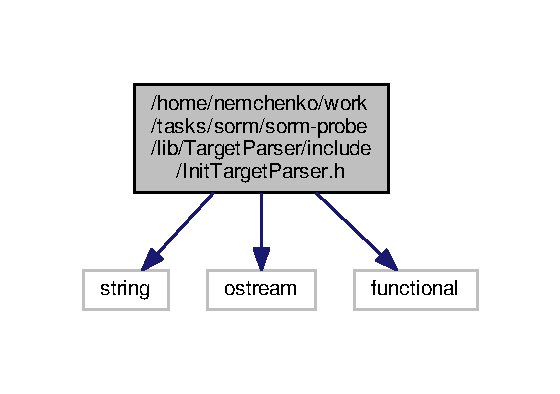
\includegraphics[width=269pt]{InitTargetParser_8h__incl}
\end{center}
\end{figure}
This graph shows which files directly or indirectly include this file\+:
\nopagebreak
\begin{figure}[H]
\begin{center}
\leavevmode
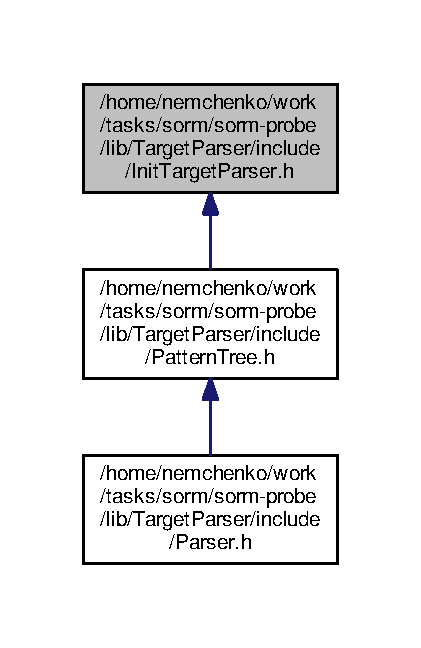
\includegraphics[width=202pt]{InitTargetParser_8h__dep__incl}
\end{center}
\end{figure}
\subsection*{Classes}
\begin{DoxyCompactItemize}
\item 
struct \hyperlink{structtarget__parser_1_1Vertex}{target\+\_\+parser\+::\+Vertex}
\begin{DoxyCompactList}\small\item\em класс представляющий терминальное состояние вершины в дереве разбора \hyperlink{classtarget__parser_1_1PatternTree}{Pattern\+Tree}. \end{DoxyCompactList}\end{DoxyCompactItemize}
\subsection*{Namespaces}
\begin{DoxyCompactItemize}
\item 
 \hyperlink{namespacetarget__parser}{target\+\_\+parser}
\begin{DoxyCompactList}\small\item\em Содержит функции и структуры для работы с парсером \end{DoxyCompactList}\end{DoxyCompactItemize}
\subsection*{Typedefs}
\begin{DoxyCompactItemize}
\item 
typedef std\+::function$<$ void(const Vertex \&)$>$ \hyperlink{namespacetarget__parser_aa28dbbced739f360834455cbffeaa6e4}{target\+\_\+parser\+::\+Func}\hypertarget{namespacetarget__parser_aa28dbbced739f360834455cbffeaa6e4}{}\label{namespacetarget__parser_aa28dbbced739f360834455cbffeaa6e4}

\begin{DoxyCompactList}\small\item\em тип функтора который передается в метод \hyperlink{classtarget__parser_1_1PatternTree_a851ee4b1279c2dcfc4557cab03f8aa83}{Pattern\+Tree\+::\+For\+Each\+Vertex}. \end{DoxyCompactList}\end{DoxyCompactItemize}
\subsection*{Functions}
\begin{DoxyCompactItemize}
\item 
void \hyperlink{namespacetarget__parser_aabf89c1d99b04bac59515c8616155d94}{target\+\_\+parser\+::\+Init} ()\hypertarget{namespacetarget__parser_aabf89c1d99b04bac59515c8616155d94}{}\label{namespacetarget__parser_aabf89c1d99b04bac59515c8616155d94}

\begin{DoxyCompactList}\small\item\em инициализирует грамматику и парсер, нужно вызывать в main до использования функции \hyperlink{namespacetarget__parser_a3e0ffa10d4fd38f05986d81c0529fdc1}{Parse }. \end{DoxyCompactList}\end{DoxyCompactItemize}


\subsection{Detailed Description}
содержит структуру Vertex и декларацию функции \hyperlink{namespacetarget__parser_aabf89c1d99b04bac59515c8616155d94}{target\+\_\+parser\+::\+Init}. 

\begin{DoxyAuthor}{Author}
Nemchenko Eugene 
\end{DoxyAuthor}
\begin{DoxyDate}{Date}
12/08/2016 
\end{DoxyDate}

\hypertarget{Parser_8h}{}\section{/home/nemchenko/work/tasks/sorm/sorm-\/probe/lib/\+Target\+Parser/include/\+Parser.h File Reference}
\label{Parser_8h}\index{/home/nemchenko/work/tasks/sorm/sorm-\/probe/lib/\+Target\+Parser/include/\+Parser.\+h@{/home/nemchenko/work/tasks/sorm/sorm-\/probe/lib/\+Target\+Parser/include/\+Parser.\+h}}


содержит декларации функций для парсинга \hyperlink{namespacetarget__parser_a3e0ffa10d4fd38f05986d81c0529fdc1}{target\+\_\+parser\+::\+Parse(char const $\ast$, size\+\_\+t, int $\ast$)}  


{\ttfamily \#include $<$string$>$}\\*
{\ttfamily \#include $<$Pattern\+Tree.\+h$>$}\\*
Include dependency graph for Parser.\+h\+:
\nopagebreak
\begin{figure}[H]
\begin{center}
\leavevmode
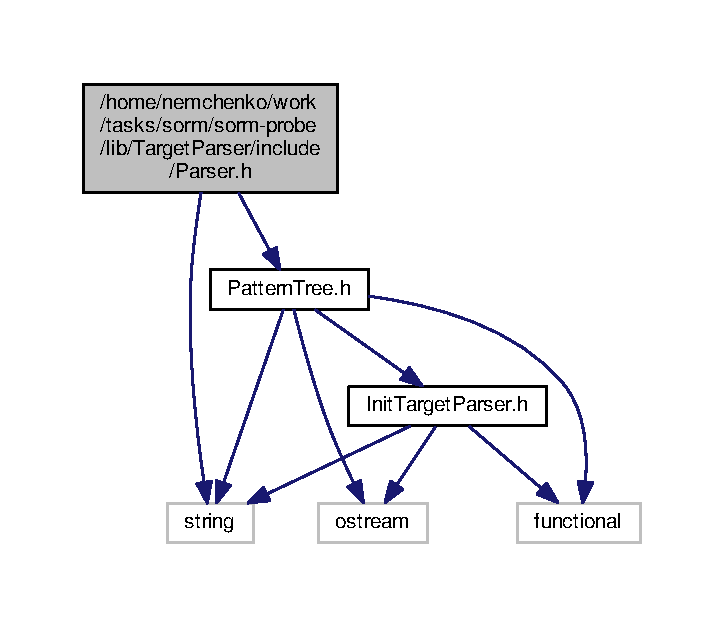
\includegraphics[width=348pt]{Parser_8h__incl}
\end{center}
\end{figure}
\subsection*{Namespaces}
\begin{DoxyCompactItemize}
\item 
 \hyperlink{namespacetarget__parser}{target\+\_\+parser}
\begin{DoxyCompactList}\small\item\em Содержит функции и структуры для работы с парсером \end{DoxyCompactList}\end{DoxyCompactItemize}
\subsection*{Functions}
\begin{DoxyCompactItemize}
\item 
Pattern\+Tree \hyperlink{namespacetarget__parser_acbab48610c44fba004e282d8008df094}{target\+\_\+parser\+::\+Parse} (const std\+::string \&text, int $\ast$pos\+\_\+unparsed=nullptr)
\item 
Pattern\+Tree \hyperlink{namespacetarget__parser_a3e0ffa10d4fd38f05986d81c0529fdc1}{target\+\_\+parser\+::\+Parse} (char const $\ast$first, size\+\_\+t len, int $\ast$pos\+\_\+unparsed=nullptr)
\begin{DoxyCompactList}\small\item\em разбирает строку по соответствующей грамматике и строит для нее дерево разбора \end{DoxyCompactList}\end{DoxyCompactItemize}


\subsection{Detailed Description}
содержит декларации функций для парсинга \hyperlink{namespacetarget__parser_a3e0ffa10d4fd38f05986d81c0529fdc1}{target\+\_\+parser\+::\+Parse(char const $\ast$, size\+\_\+t, int $\ast$)} 

\begin{DoxyAuthor}{Author}
Nemchenko Eugene 
\end{DoxyAuthor}
\begin{DoxyDate}{Date}
12/08/2016 
\end{DoxyDate}

\hypertarget{PatternTree_8h}{}\section{/home/nemchenko/work/tasks/sorm/sorm-\/probe/lib/\+Target\+Parser/include/\+Pattern\+Tree.h File Reference}
\label{PatternTree_8h}\index{/home/nemchenko/work/tasks/sorm/sorm-\/probe/lib/\+Target\+Parser/include/\+Pattern\+Tree.\+h@{/home/nemchenko/work/tasks/sorm/sorm-\/probe/lib/\+Target\+Parser/include/\+Pattern\+Tree.\+h}}


содержит класс представляющий дерево разбора \hyperlink{classtarget__parser_1_1PatternTree}{target\+\_\+parser\+::\+Pattern\+Tree}.  


{\ttfamily \#include $<$string$>$}\\*
{\ttfamily \#include $<$ostream$>$}\\*
{\ttfamily \#include $<$functional$>$}\\*
{\ttfamily \#include $<$Init\+Target\+Parser.\+h$>$}\\*
Include dependency graph for Pattern\+Tree.\+h\+:
\nopagebreak
\begin{figure}[H]
\begin{center}
\leavevmode
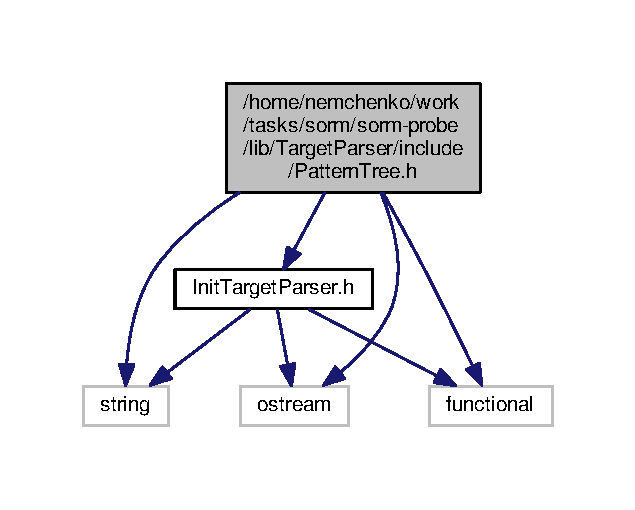
\includegraphics[width=305pt]{PatternTree_8h__incl}
\end{center}
\end{figure}
This graph shows which files directly or indirectly include this file\+:
\nopagebreak
\begin{figure}[H]
\begin{center}
\leavevmode
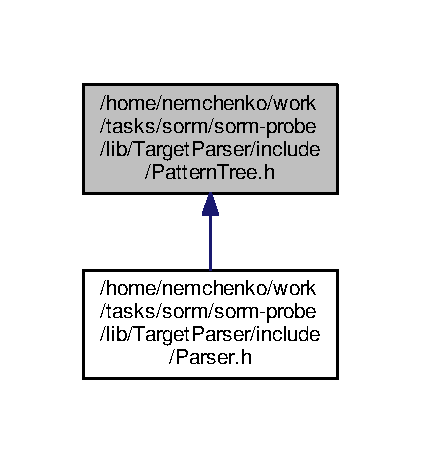
\includegraphics[width=202pt]{PatternTree_8h__dep__incl}
\end{center}
\end{figure}
\subsection*{Classes}
\begin{DoxyCompactItemize}
\item 
class \hyperlink{classtarget__parser_1_1PatternTree}{target\+\_\+parser\+::\+Pattern\+Tree}
\begin{DoxyCompactList}\small\item\em Класс представляющий разобранное выражение в виде дерева, возвращается из метода \hyperlink{namespacetarget__parser_a3e0ffa10d4fd38f05986d81c0529fdc1}{Parse }. \end{DoxyCompactList}\end{DoxyCompactItemize}
\subsection*{Namespaces}
\begin{DoxyCompactItemize}
\item 
 \hyperlink{namespacetarget__parser}{target\+\_\+parser}
\begin{DoxyCompactList}\small\item\em Содержит функции и структуры для работы с парсером \end{DoxyCompactList}\end{DoxyCompactItemize}


\subsection{Detailed Description}
содержит класс представляющий дерево разбора \hyperlink{classtarget__parser_1_1PatternTree}{target\+\_\+parser\+::\+Pattern\+Tree}. 

\begin{DoxyAuthor}{Author}
Nemchenko Eugene 
\end{DoxyAuthor}
\begin{DoxyDate}{Date}
12/08/2016 
\end{DoxyDate}

%--- End generated contents ---

% Index
\backmatter
\newpage
\phantomsection
\clearemptydoublepage
\addcontentsline{toc}{chapter}{Index}
\printindex

\end{document}
